% Part: sets-functions-relations
% Chapter: infinite
% Section: hilberts-hotel
%
\documentclass[../../../include/open-logic-section]{subfiles}

\begin{document}

\olfileid[id]{sfr}{infinite}{hilbert}
\olsection{Hotel Hilbert}

Himpunan bilangan asli jelas bersifat tak hingga. Jadi, jika kita tidak ingin
begitu saja \emph{mengandaikan tersedianya} bilangan asli, langkah pertama
kita harus mencirikan himpunan tak hingga dengan istilah yang tidak perlu
menyebut bilangan asli itu sendiri. Berikut suatu pendekatan yang elok,
disampaikan Hilbert dalam sebuah kuliah pada tahun 1924. Ia meminta kita
membayangkan
\begin{quote}
[\ldots] sebuah hotel dengan sejumlah hingga kamar. Setiap kamar itu harus
dihuni tepat oleh satu tamu. Jika para tamu kemudian saling bertukar kamar
dengan suatu cara, [tetapi] sedemikian sehingga setiap kamar tetap dihuni
tidak lebih dari satu orang, tidak ada kamar yang akan menjadi kosong, dan
dengan cara ini pemilik hotel tidak dapat menciptakan tempat baru bagi tamu
yang baru datang [\ldots
\textparagraph \ldots]

Sekarang kita tetapkan bahwa hotel itu mempunyai kamar-kamar bernomor yang
banyaknya tak hingga, $1$, $2$, $3$, $4$, $5$, \dots, dan masing-masing
dihuni tepat oleh satu tamu. Begitu seorang tamu baru datang, pemilik hanya
perlu memindahkan setiap tamu lama ke kamar yang nomornya satu lebih besar,
dan kamar~$1$ akan kosong bagi tamu yang baru datang itu.
	\begin{center}
		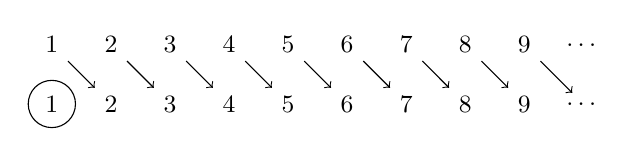
\begin{tikzpicture}[scale = .75]
		\foreach \x in {1, 2, 3, 4, 5, 6, 7, 8, 9}
		{
			\node (\x a) at (\x, 1) {\small{\x}};
			\node (\x b) at (\x, 2) {\small{\x}};
		}
		\node (dotsa) at (10, 1) {\small{\ldots}};
		\node (dotsb) at (10, 2) {\small{\ldots}};
		\draw[->] (1b)--(2a);
		\draw[->] (2b)--(3a);
		\draw[->] (3b)--(4a);
		\draw[->] (4b)--(5a);
		\draw[->] (5b)--(6a);
		\draw[->] (6b)--(7a);
		\draw[->] (7b)--(8a);
		\draw[->] (8b)--(9a);
		\draw[->] (9b)--(dotsa);
		\draw (1,1) circle (.4);
		\end{tikzpicture}
	\end{center}
	(diterbitkan dalam \citealt[730]{EwaldSieg2013}; terjemahan kami)
\end{quote}
Pokok yang menentukan ialah bahwa Hotel Hilbert mempunyai kamar yang
banyaknya tak hingga; dan penjelasannya dapat kita gunakan untuk
mendefinisikan arti pernyataan tersebut. Memang, inilah pendekatan Dedekind
(tentu saja disajikan di sini dengan anakronisme yang sangat besar; definisi
Dedekind berasal dari \citeyear{Dedekind1888}):

\begin{defn}\ollabel{defn:DedekindInfinite}
Suatu himpunan $A$ bersifat \emph{tak hingga Dedekind} jika dan hanya jika
terdapat !!a{injection} dari~$A$ ke suatu himpunan bagian sejati dari~$A$.
Artinya, terdapat suatu $o \in A$ dan !!a{injection} $f \colon A \to A$
sedemikian sehingga $o \notin \ran{f}$.
\end{defn}

\end{document}
